\section{Abstract}
Dieser Versuch beschäftigt sich mit der optischen Fouriertransformation eines Laserstrahls an einem Objekt und den Möglichkeiten, die sich daraus ergeben. Zuerst wird das Interferenzbild eines Gitters in unterschiedlichen Entfernungen betrachtet, um so den Übergang von der Fresnel- zur Fraunhoferbeugung darzustellen. Anschließend werden die Gitterkonstanten fünf verschiedener Gitter mithilfe des Abstands der Beugungsmaxima im Fernfeld bestimmt.

\section{Methoden}
Die optische Fouriertransformation wird in diesem Versuch mit einem Helium-Neon-Laser durchgeführt. Dieser strahlt entlang einer optischen Bank, auf der verschiedene optische Instrumente befestigt sind, auf eine Kamera. Das Bild der Kamera wird direkt auf einen Computer übertragen. Zur Fouriertransformation wird ausgenutzt, dass das Beugungsbild eines Objekts im Unendlichen die Fouriertransformation ist. Mithilfe einer Linse kann die Fouriertransformation in der Brennebene der Linse sichtbar gemacht werden. Dieser Aufbau wird auch als 2-f-Aufbau bezeichnet. Wird hinter der Brennebene der ersten Linse eine zweite Linse aufgestellt, wird die Fouriertransformation rückgängig gemacht und in der Brennebene der zweiten Linse wird das ursprüngliche Bild wieder sichtbar. Dies ist unter dem Namen 4-f-Aufbau bekannt. Wird nun in der Fourierebene ein Teil des Strahls geblockt, werden einzelne Frequenzen des Bildes gefiltert. Diesen Vorgang bezeichnet man als optische Fourierfilterung.

\section{Theorie}
Um die Vorgänge an einem Gitter im Nah- bzw. Fernfeld zu beschreiben wird die skalare Beugungstheorie herangezogen. Dabei entsteht nach dem Huygenschen Prinzip Elementarwellen, welche kohärent sind. Diese interferieren konstruktiv oder destruktiv miteinander. Die Beobachtungen von Interferenz an einem Spalt können durch die Fresnel- und Frauenhofertheorie beschrieben werden. \cref{Theoriebild} zeigt die grafischen Verläufe.
\begin{figure}[h!]
	\centering
	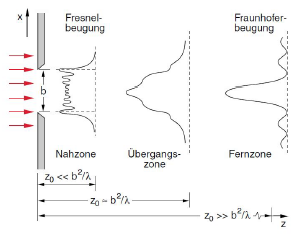
\includegraphics[scale = 1.5]{abstande.png}
	\caption{Fresnel- und Frauenhofer Näherung. Im Fernfeld kann die Frauenhofer Näherung angewandt werden, wohingegen im Nahfeld die Fresnel Näherung angewandt wird.}
	\label{Theoriebild}
\end{figure}
In der Nahzone wird die Interferenz durch die Fresnel-Näherung beschrieben, wohingegen die Interferenz im Fernfeld über die Frauenhofer Näherung beschrieben wird. Die Fresnel-Näherung kann angenommen werden, wenn der Abstand der Lichtquelle zum Beugungsobjekt groß gegenüber der Ausdehnung des Beugungsobjektes (b) ist. Ist hingegen der Abstand vom Schirm zum Beugungsobjekt groß kann die Frauenhofer Näherung angewandt werden.

\section{Übergang von Nah- zu Fernfeld}
In diesem Versuchsteil wird das Beugungsbild eines Gitters in Abhängigkeit des Abstandes zwischen Schirm und Gitter beobachtet. Dabei wird ein kollimierter Laserstrahl mit einer Wellenlänge von $\lambda = 633 nm$ auf einen Schirm gerichtet. Der Laserstrahl wird, um ihn zu kollimieren, auf zwei Linsen gerichtet. Die erste Linse weitet den Stahl auf und die zweite Linse fokussiert den Strahl wieder. Der Abstand der Linsen beträgt gerade die Summe der beiden Brennweiten der Linsen. Zwischen den beiden Linsen wird ein Gitter in den Strahlengang gesetzt, sodass das Gitter komplett beleuchtet wird. Mit diesem Aufbau kann nun das Beugungsbild bei unterschiedlichem Abstand zwischen Schirm und Gitter beobachtet werden. \cref{alle} zeigt den Verlauf der Beugungsbilder bei veränderlichem Abstand. Je größer der Abstand vom Schirm zum Gitter wird, desto kleiner wird der Abstand zwischen Gitter und Laser. Je näher sich das Gitter zum Laser bewegt, desto mehr wird sich das Fernfeld einstellen.

\begin{figure}[h!]
	\centering
	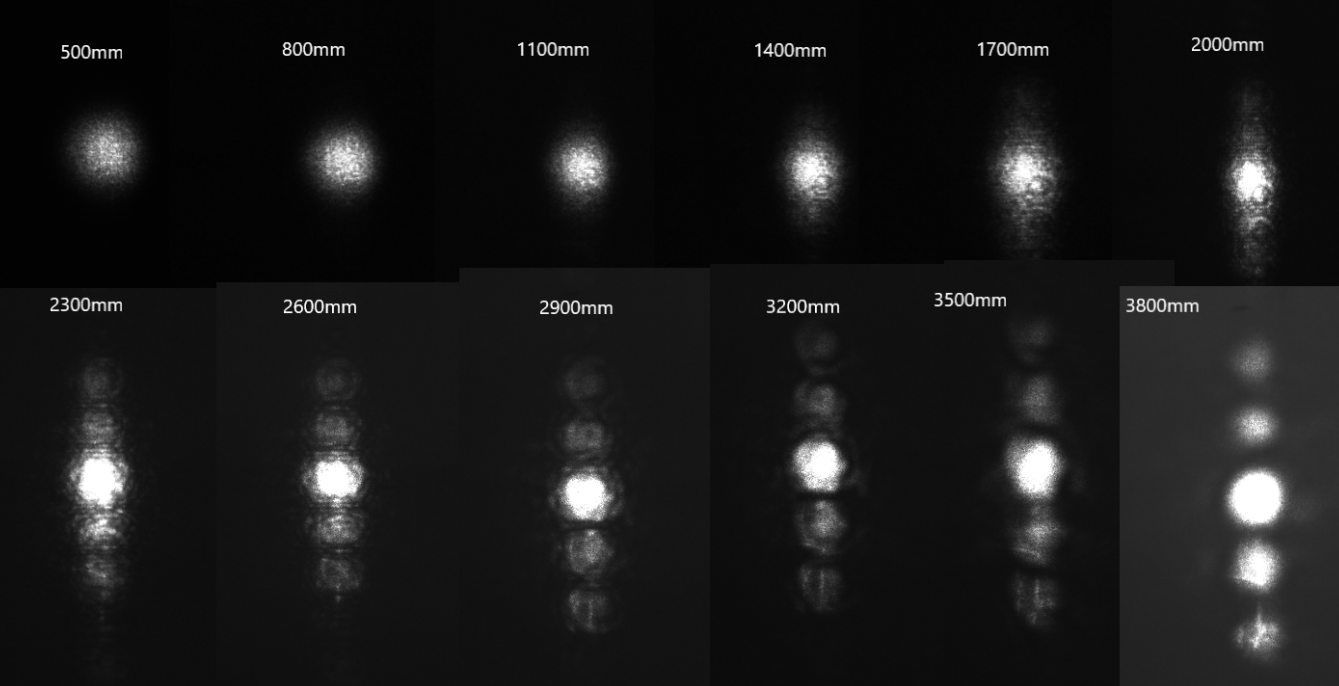
\includegraphics[scale = 0.65]{alleabstande.png}
	\caption{Es sind die Beugungsbilder in Abhängigkeit der Abstände zwischen Schirm und Gitter aufgetragen. Oben Links ist das Beugungsbild im Nahfeld zu erkennen bei einem Abstand von 500mm. Unten rechts ist das Beugungsbild im Fernfeld zu erkennen bei einem Abstand von 3800mm. Von oben links nach unten rechts nimmt der Abstand zu. Der Abstand nimmt in 300mm Abständen zu.}
	\label{alle}
\end{figure}
In \cref{alle} kann in einem Abstand von $500 mm$ bis $1400 mm$ das Nahfeld erkannt werden. Bei einem Abstand von $1700 mm$ bis $2600 mm$  kann das Übergangsfeld beobachtet werden und in einem Abstand von $2900 mm$ bis $3800 mm$ kann das Fernfeld beobachtet werden. Die angegebenen Grenzen sind keine scharfen Grenzen. Häufig kann man an den Grenzen beide Effekte erkennen. Die Effekte sind beim Nah- und Fernfeld vor allem an den Rändern sichtbar (also bei $500 mm$ bzw. bei $3800 mm$) und beim Übergangsfeld bei einem Abstand von $2000 mm$. Diese Angaben wurden mit \cref{Theoriebild} erhoben. Gründe für diese Einteilung sind, dass sich die Maxima höherer Ordnung erst im Fernfeld klar unterscheiden lassen und sich die Maxima im Nahfeld in einem Punkt treffen. Charakteristisch für die Übergangszone ist das vermischen beider Effekte. Das Hauptmaxima ist deutlich zu erkennen, jedoch gibt es entfernt vom Hauptmaxima noch Helligkeitserscheinungen, die nach außen hin abschwächen und kaum zu erkennende Peaks ausbilden. Diese Charakteristiken können im Vergleich von \cref{Theoriebild} und \cref{alle} an den oben genannten Bildern beobachtet werden.

\section{Bestimmung der Gitterkonstanten}
In diesem Abschnitt wurden die Gitterkonstanten verschiedener Gitter bestimmt. Dafür wurde das Gitter in den Strahlengang gestellt. Die Kamera wird $\SI{3800}{mm}$ entfernt positioniert. Das Beugungsbild von Gitter 5 ist exemplarisch in \cref{Gitter5} dargestellt.

\begin{figure}
	\centering
	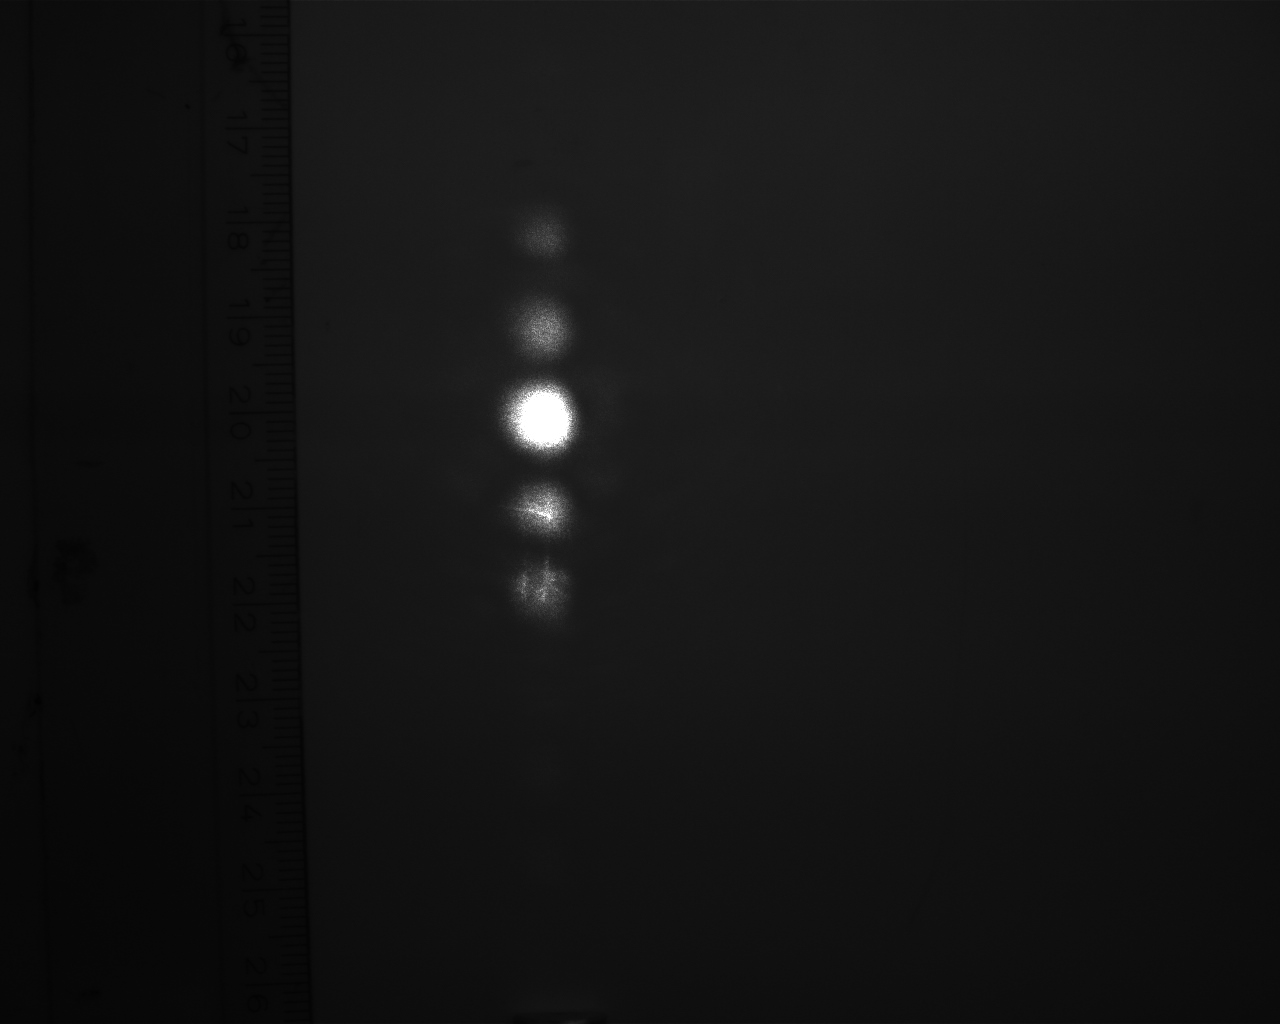
\includegraphics[scale=0.4]{Gitter5.jpg}
	\caption{Das Beugungsbild des 5. Gitters.}
	\label{Gitter5}
\end{figure}

Aus dem Abstand der einzelnen Beugungsmaxima zum nullten Beugungsmaximum $a$ und dem Abstand zwischen Gitter und Kamera $d$ kann dann mit \cref{eq:sin} $\theta$ bestimmt werden.

\begin{equation}
	\theta = \arctan\left(\frac{a}{d}\right)
	\label{eq:sin}
\end{equation}

Nun lässt sich die Gitterkonstante des untersuchten Gitters mit \cref{eq:gk} bestimmen, mit $k$ der Nummer des Beugungsmaximums.

\begin{equation}
	k\lambda = b \sin(\theta)
	\label{eq:gk}
\end{equation}

Bei jedem Gitter wurde die Gitterkonstante jeweils viermal bestimmt, mit den beiden ersten Beugungsmaxima nach oben und unten ausgehend vom nullten Maximum. Aus diesen wurde dann der Mittelwert gebildet. Die Ergebnisse sind in \cref{tab} zusammengefasst.

\begin{table}[h]
	\caption{Die Gitterkonstanten der fünf untersuchten Gitter in mm}
\begin{tabular}{lllll}
	Gitter 1 & Gitter 2& Gitter 3& Gitter 4& Gitter 5\\
	 $0,386\pm0,048$ & $0,456\pm0,053$ & $0,363\pm0,041$ & $0,323\pm0,032$ & $0,252\pm0,020$
\end{tabular}
\label{tab}
\end{table}

Die Unsicherheit beim Ablesen der Abstände wurde auf $\SI{\pm1}{mm}$ geschätzt. Daraus ergibt sich mithilfe der Formel für die Fehlerfortpflanzung (\cref{eq:utheta}) die Unsicherheit von $\theta$ und daraus mit \cref{eq:ugk} die Gesamtunsicherheit der Gitterkonstanten.

\begin{align}
u(\theta) &= \frac{u(a)*d}{a^2 +d^2}
\label{eq:utheta}\\
u(b) &= \frac{u(\theta) k \lambda \cos(\theta)}{sin(\theta)^2}
\label{eq:ugk}
\end{align}

\section{Fourierfilterung}
\subsection{Ergebnis}
\subsection{Fourier Schriftzug}
Zuerst soll ein "Fourier" Schriftzug vor einem Gitter modelliert werden, indem das Gitter entfernt wird. Dazu wird eine Tiefpassfilterung benutzt, da die im Vergleich große Schrift hauptsächlich aus niedrigen Frequenzen besteht. 


\begin{figure}[h]
\begin{subfigure}[c]{0.5\textwidth}

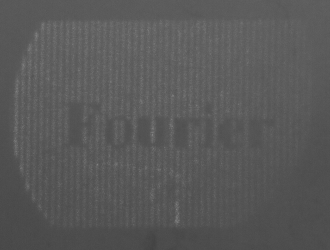
\includegraphics[width=0.9\textwidth]{Fourier.png}
	      \caption{}
          \label{fig:NiceImage1}
          
\end{subfigure}
\begin{subfigure}[c]{0.5\textwidth}
	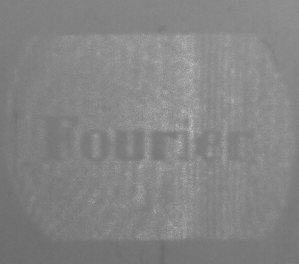
\includegraphics[width=0.9\textwidth]{Fourier_Filter.png}
	      \caption{}
          \label{fig:NiceImage2}
\end{subfigure}
\caption{In \cref{fig:NiceImage1} ist der "Fourier" Schriftzug ohne Filter zu sehen; in \cref{fig:NiceImage2} mit einem Tiefpassfilter.}
\label{Fourier}
\end{figure}   

In \cref{Fourier} ist zu sehen, wie sich der Tiefpassfilter auf das Bild auswirkt. Das Gitter ist zum größten Teil nicht mehr als solches zu erkennen.

\subsection{Nenner eines Bruches entfernen}
Daraufhin soll der Nenner eines $\frac{1}{2}$ Bruchs entfernt werden. Wie in \cref{fig:Bruch} zu sehen ist, befindet sich unter dem Zähler ein Gitter, welches sich nicht bei dem Nenner befindet. Es werden also praktisch beide Zahlen entfernt, allerdings ist durch das Gitter immer noch der Umriss der 1 sichtbar. Dieses entfernen geschieht durch eine Hochpassfilterung, was bedeutet, dass niedrige Frequenzen entfernt werden. Das hat sehr gut funktioniert, da in \cref{fig:Bruch_filter} die Zwei, also der Nenner nicht mehr erkennbar ist.

\begin{figure}[h]
	\begin{subfigure}[c]{0.5\textwidth}
		
		\includegraphics[width=0.6\textwidth]{Bruch.png}
		\caption{}
		\label{fig:Bruch}
		
	\end{subfigure}
	\begin{subfigure}[c]{0.5\textwidth}
		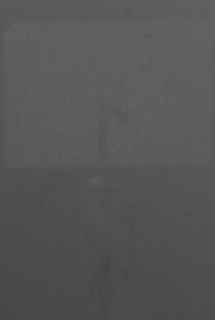
\includegraphics[width=0.58\textwidth]{Filter_Bruch.png}
		\caption{}
		\label{fig:Bruch_filter}
	\end{subfigure}
	\caption{In \cref{fig:Bruch} ist der $\frac{1}{2}$ Bruch ohne Filter zu sehen; in \cref{fig:Bruch_filter} mit einem Hochpassfilter, wodurch die Zwei entfernt wurde.}
	\label{Bruch}
\end{figure}   

\subsection{Tiefpassfilterung bei einem Quadratgitter}
Als nächstes soll ausprobiert werden, was passiert, wenn ein Quadratgitter eingesetzt wird, das mit einem eindimensionalem Tiefpassfilter in verschiedenen Ausrichtungen gefiltert wird. Das ungefilterte Bild ist in \cref{fig:Gitter} zu sehen. Dazu im Vergleich wurde in \cref{fig:0Gitter} ein Tiefpassfilter im Winkel von 0° Grad eingebaut. Da der Tiefpass alle Frequenzen außer denen, die im 0° Winkel sind durchgelassen. Deshalb wurde erwartet, dass die Linien orthogonal zum Frequenzbild erkennbar sind. Allerdings ist das besonders am Rand und zum Teil auch in der Mitte des Bildes nicht immer deutlich zu erkennen. 

Ähnliche Probleme gibt es auch in \cref{fig:45Gitter} und \cref{fig:90Gitter}, in denen der Tiefpassfilter jeweils um 45° und 90° gedreht sind. Besonders in \cref{fig:45Gitter} lässt sich die Ausrichtung nur noch erahnen, während bei der 90° Drehung das Muster nur in der Mitte des Bildes unterbrochen wird.

Diese hellen Strahlen, die sich an der räumlichen Ausrichtung des Filters orientieren und damit die erwarteten Muster unterbrechen, stammen höchstwahrscheinlich daher, dass der Tiefpassfilter sich beim Messen nicht perfekt in der Fourierebene befand. Trotzdem lässt sich bei genauerem Hinschauen das erwartete Muster erkennen.





\begin{figure}[h]
	\begin{subfigure}[c]{0.5\textwidth}
		
		\includegraphics[width=1\textwidth]{Quadratgitter.png}
		\caption{}
		\label{fig:Gitter}
		
	\end{subfigure}
	\begin{subfigure}[c]{0.5\textwidth}
		\includegraphics[width=1\textwidth]{0Grad_Tiefpass_quadrat.png}
		\caption{}
		\label{fig:0Gitter}
	\end{subfigure}
	\caption{In \cref{fig:Gitter} ist das Quadratgitter ohne einen Filter zu sehen; in \cref{fig:0Gitter} mit einem Tiefpassfilter im 0° Winkel}
	\label{Gitter1}
\end{figure}  




\begin{figure}[h]
	\begin{subfigure}[c]{0.5\textwidth}
		
		\includegraphics[width=1\textwidth]{45Grad_Tiefpass_quadrat.png}
		\caption{}
		\label{fig:45Gitter}
		
	\end{subfigure}
	\begin{subfigure}[c]{0.5\textwidth}
		\includegraphics[width=1\textwidth]{90Grad_Tiefpass_quadrat.png}
		\caption{}
		\label{fig:90Gitter}
	\end{subfigure}
	\caption{In \cref{fig:45Gitter} ist das Quadratgitter mit einem Tiefpassfilter im 45° Winkel zu sehen; in \cref{fig:90Gitter} im 90° Winkel.}
	\label{blabla}
\end{figure}  




\subsection{Hochpassfilterung einer Schraube}
Daraufhin wird eine Schraube einer Hochpassfilterung unterzogen. In \cref{Schraube} sind die Bilder mit und ohne Filter zu sehen. In \cref{fig:Schraube_Filter} ist dabei nur noch der Umriss der Schraube zu sehen. Da sowohl der Laser selbst als auch die Schraube selbst nahezu homogen sind, werden dafür fast nur niedrige Frequenzen benutzt. Der Rand der Schraube hat allerdings mehre kleine Kanten, die durch hohe Frequenzen dargestellt werden und deshalb durch den Hochpassfilter durchkommen.

\begin{figure}[h]
	\begin{subfigure}[c]{0.5\textwidth}
		
		\includegraphics[width=1\textwidth]{Schraube_ohneFilter.png}
		\caption{}
		\label{fig:Schraube}
		
	\end{subfigure}
	\begin{subfigure}[c]{0.5\textwidth}
		\includegraphics[width=1\textwidth]{Schraube.png}
		\caption{}
		\label{fig:Schraube_Filter}
	\end{subfigure}
	\caption{In \cref{fig:Schraube} ist die Schraube ohne Filter zu sehen, in \cref{fig:Schraube_Filter} wurde noch ein Hochpassfilter benutzt.}
	\label{Schraube}
\end{figure}  

\subsection{Dunkelfeldmethode}
Zuletzt soll noch die Dunkelfeldmethode getestet, die Luftströme sichtbar machen kann. Dazu wird ein Teelicht 

\begin{figure}[h!]
	\centering
	\includegraphics[scale = 1]{Flamme.png}
	\caption{}
	\label{Flamme}
\end{figure}
